\chapter{Time Series}

\section{Fourier Series}

La serie de Fourier es un proceso analítico que permite representar una función $f(t)$ en base a funciones sinusoidales, es decir, 

$$
f(t) = a_0/2 + \sum_{n=1}^{\infty} (a_n \cos(nt) + b_n \sin(nt))
$$
y el objetivo es determinar los coeficientes $a_n$ y $b_n$ que hacen esto posible. Se puede mostrar que
\begin{equation*}
\begin{aligned}
a_0 &= \frac{1}{\pi}\int_{-\pi}^{\pi} f(t)dt \\
a_n &= \frac{1}{\pi}\int_{-\pi}^{\pi} f(t)cos(nt)dt \quad \forall n > 0 \\ 
b_n &= \frac{1}{\pi}\int_{-\pi}^{\pi} f(t)sin(nt)dt \quad \forall n > 0
\end{aligned}
\end{equation*}

También es posible reescribir esta ecuación mediante notación compleja según 
$$ 
f(t) = \sum_{-\infty}^{\infty} c_n e^{int}
$$
Donde los coeficientes $c_n$ se calculan según 
$$
c_n = \frac{1}{2\pi}\int_{-\pi}^{\pi}f(t)e^{-int}dt
$$

Esta descomposición es especialmente útil para suavizar funciones al truncar la cantidad de términos sinusoidales de la serie de Fourier. 

\begin{figure}[H]
    \center
    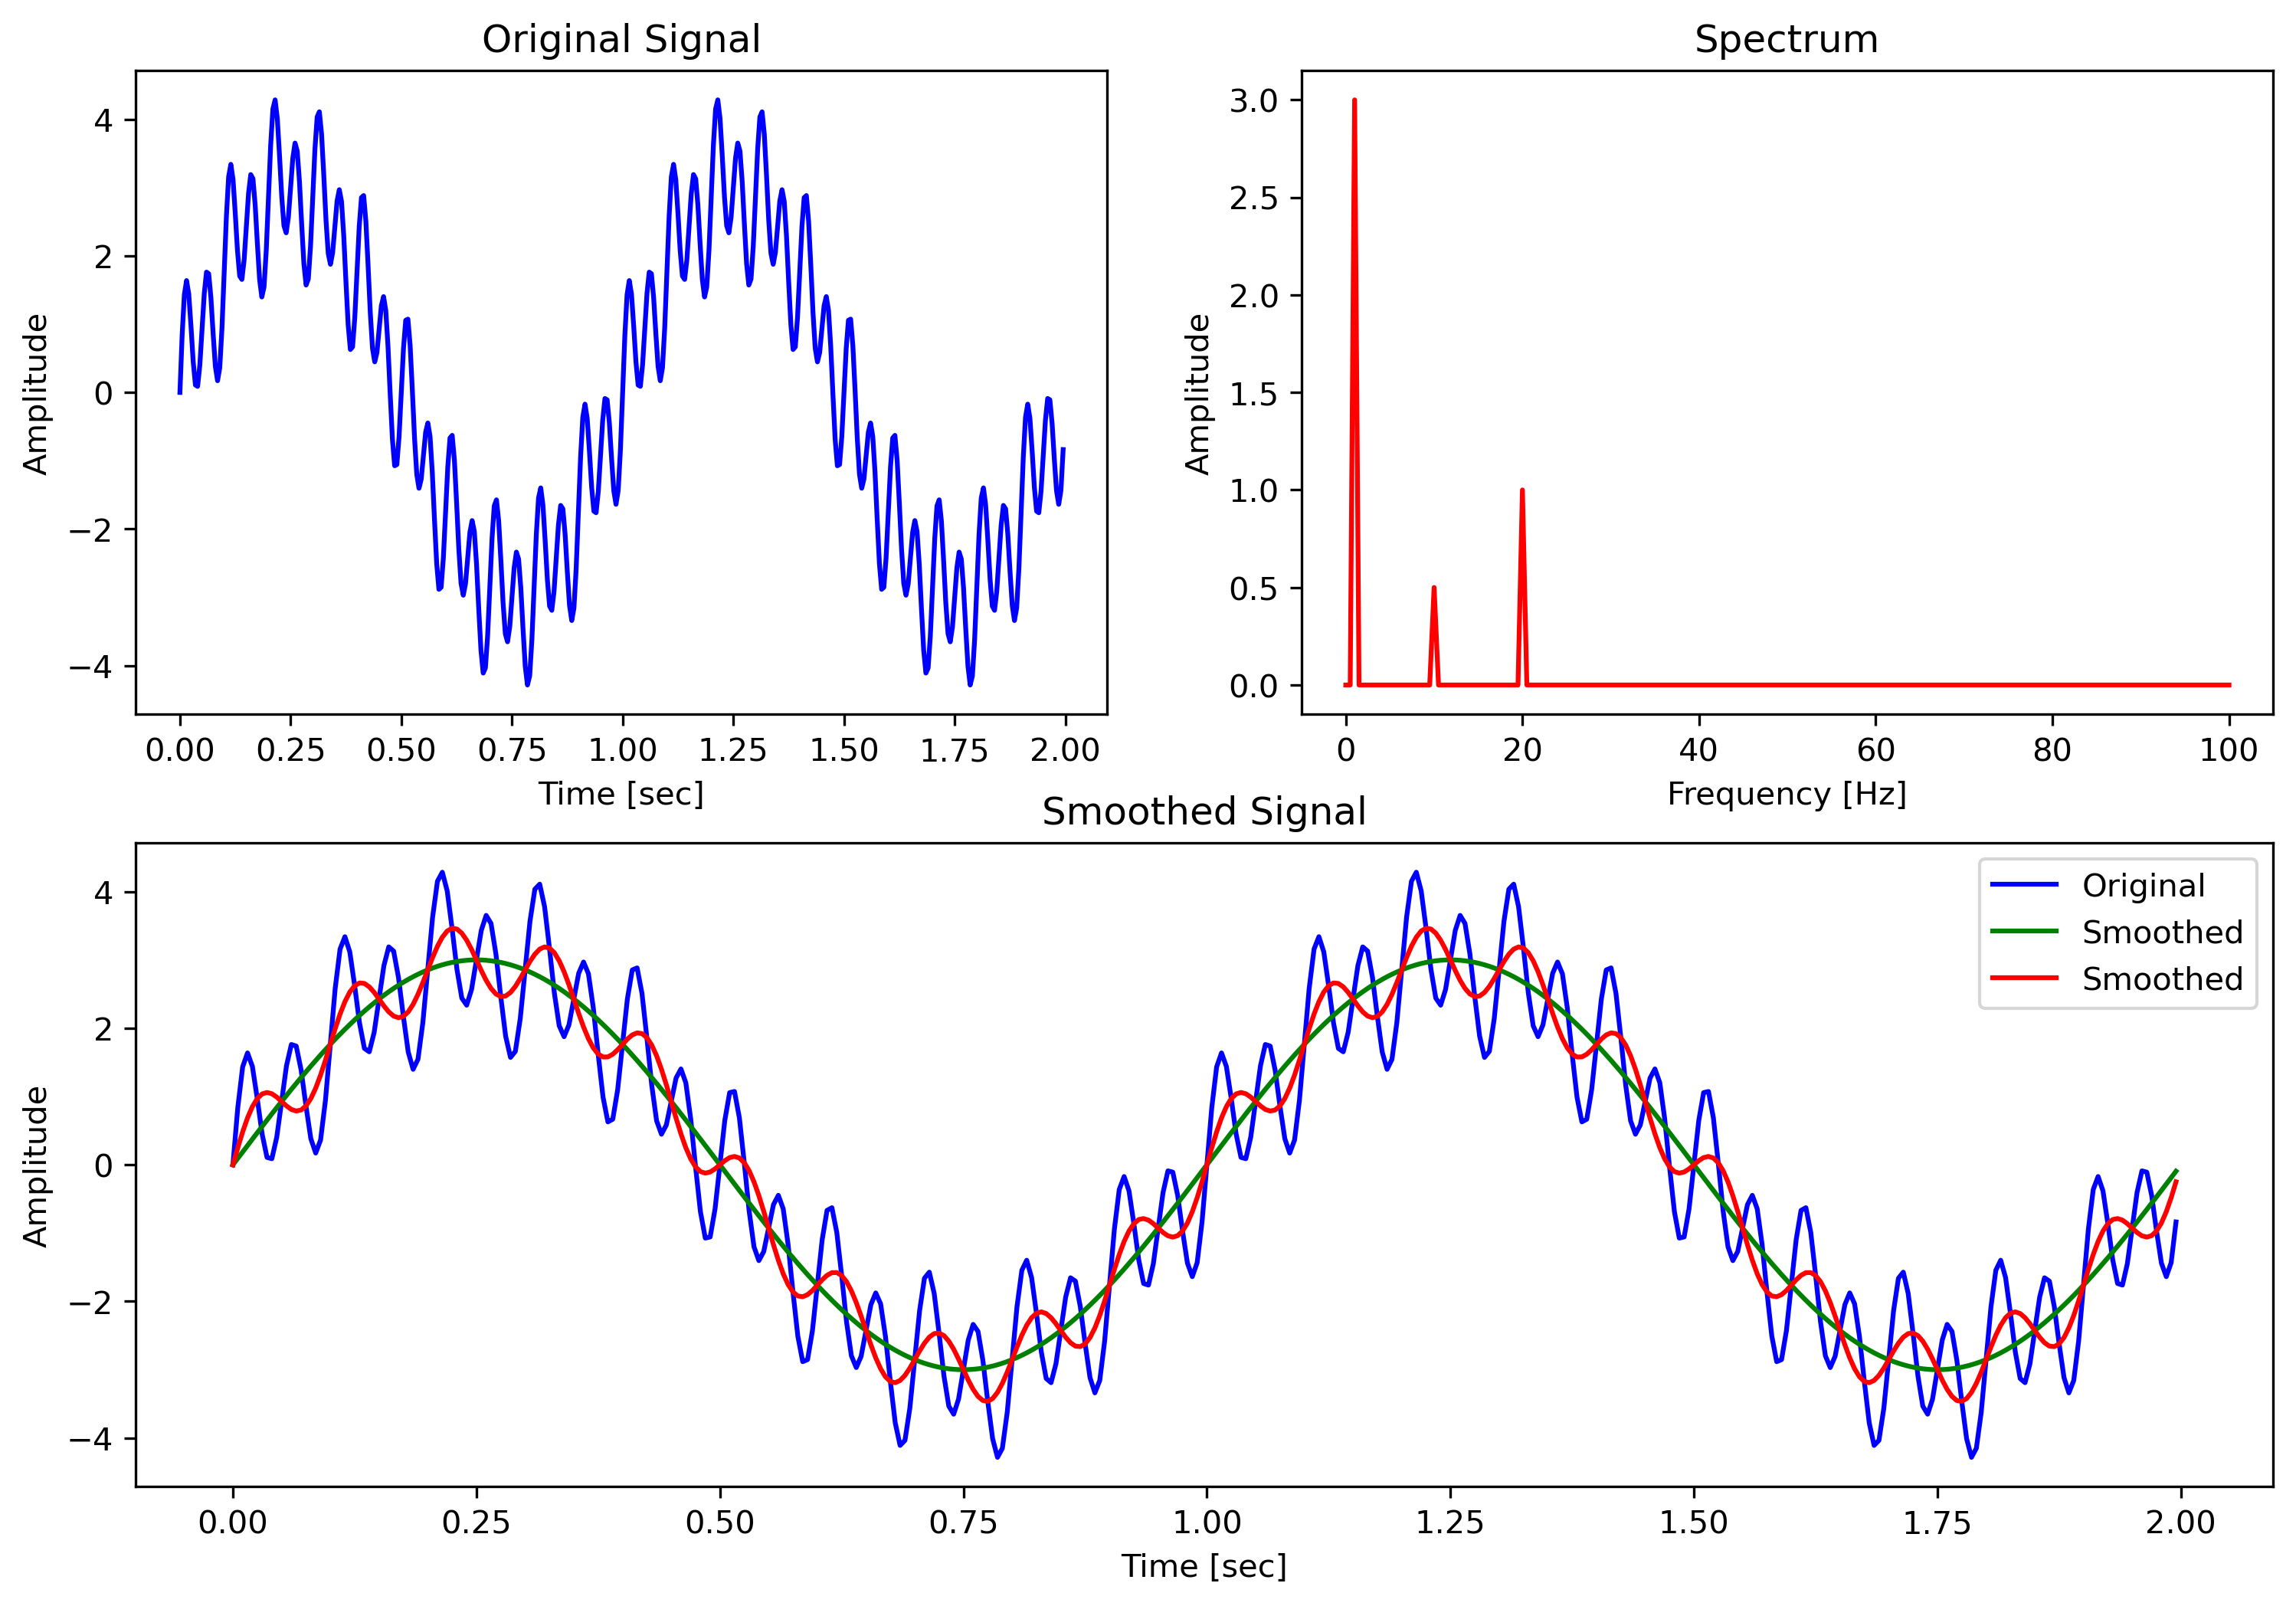
\includegraphics[scale=0.5]{notebooks/TS/img/fourier_transform_smoothing.png}
    \caption{Fourier Transform Smoothing}
\end{figure}

\section{ARIMA}

ARIMA es la abreviación de \textit{Auto-Regressive Integrated Moving Average} y es un método estadístico para realizar forecasting sobre series de tiempo que integra los siguientes conceptos:

\begin{enumerate}
    \item Toma en consideración patrones de crecimiento/decrecimiento en la serie de tiempo (\textit{Auto-Regressive}). 
    \item Estima tasa de crecimiento/decrecimiento (\textit{Integrated}).
    \item Controla el ruido entre datos consecutivos en el tiempo (\textit{Moving Average}).
\end{enumerate}

La fórmula general para este tipo de modelos viene dada por 
$$
Y_t = c + \phi_1y^d_{t-1} + \dots + \phi_py^d_{t-p} + \theta_1e_{t-1} + \dots + \theta_q e_{t-q} + e_t
$$
Aquí $c$ es una constante y $e$ es un término de error. Los modelos de este tipo son escritos como ARIMA($p,d,q$) donde: 

\begin{itemize}
    \item $p$ es la cantidad de tiempos en que la variable es mirada al pasado (Lag).
    \item $d$ es la cantidad de veces que la variable es diferenciada para producir una señal estacionaria. $d=0$ refiere a que la señal ya es estacionaria, $d=1$ es que la señal crece/decrece linealmente y $d=2$ es que la señal crece exponencialmente. 
    \item $q$ representa la cantidad de lag para el término de error $e$, esto captura el \textit{Moving Average}.
\end{itemize}

\subsection{P Value}

En la práctica, es posible determinar el valor de $p$ a través del \textit{Partial Autocorrelation Plot}. Este gráfico muestra la relación de un valor en la serie de tiempo con \textbf{un solo lag} (eliminando relaciones de tiempos intermedios ajustando una regresión lineal y quedándose sólo con el parámetro correspondiente).
\begin{figure}[H]
    \center
    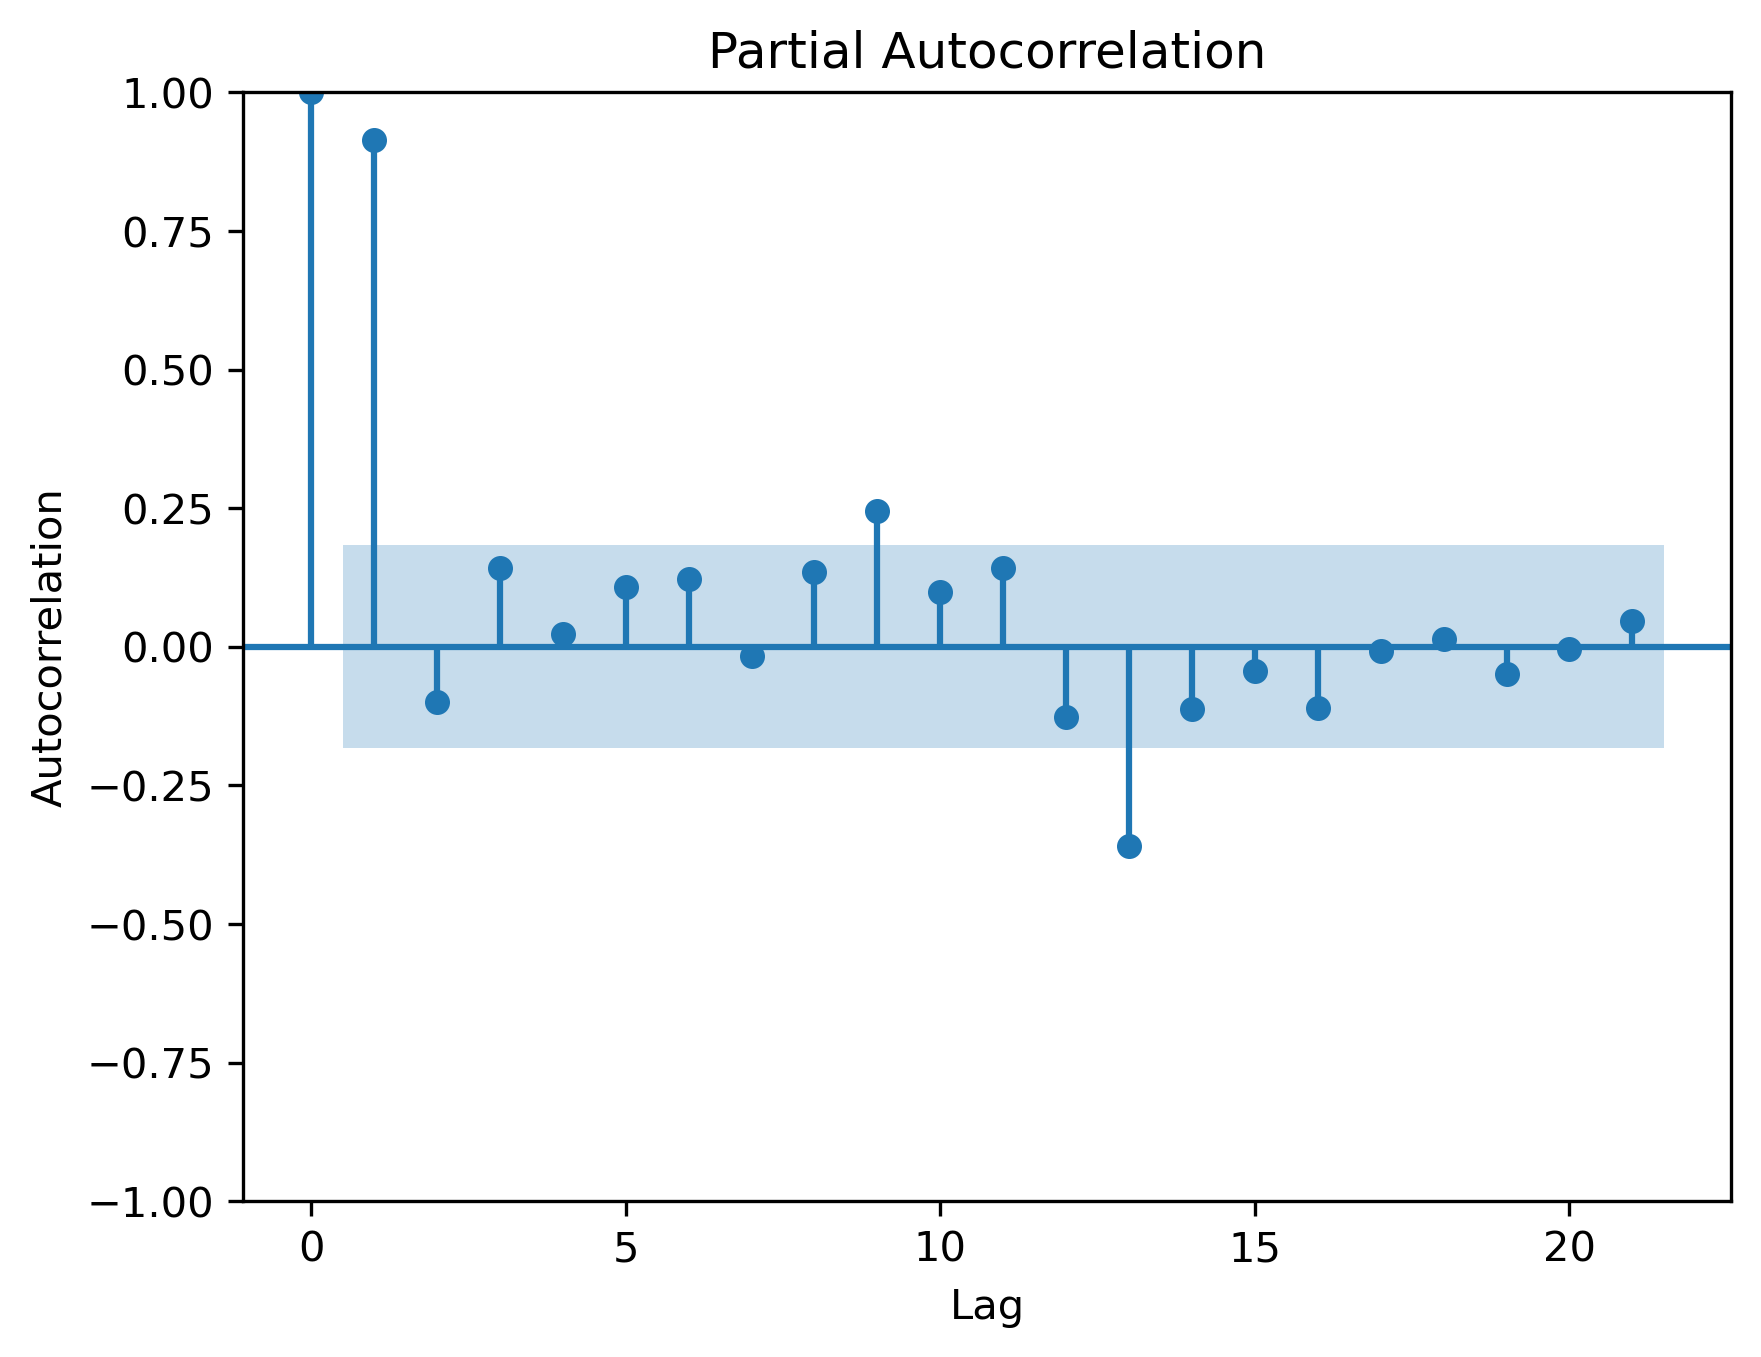
\includegraphics[scale=0.5]{notebooks/TS/img/partial_autocorrelation.png}
    \caption{Partial Autocorrelation Plot}
\end{figure}
El valor óptimo es el último punto después del cual todos los lags están dentro de las bandas azules (intervalos de confianza), en este caso $p=13$. 

\subsection{D Value}

El valor de $d$ se puede calcular diferenciando la serie de tiempo hasta encontrar una serie estacionaria. Esto lo podemos medir con un test estadístico de estacionalidad (\textit{Augmented Dickey Fuller Test}).

\begin{figure}[H]
    \center
    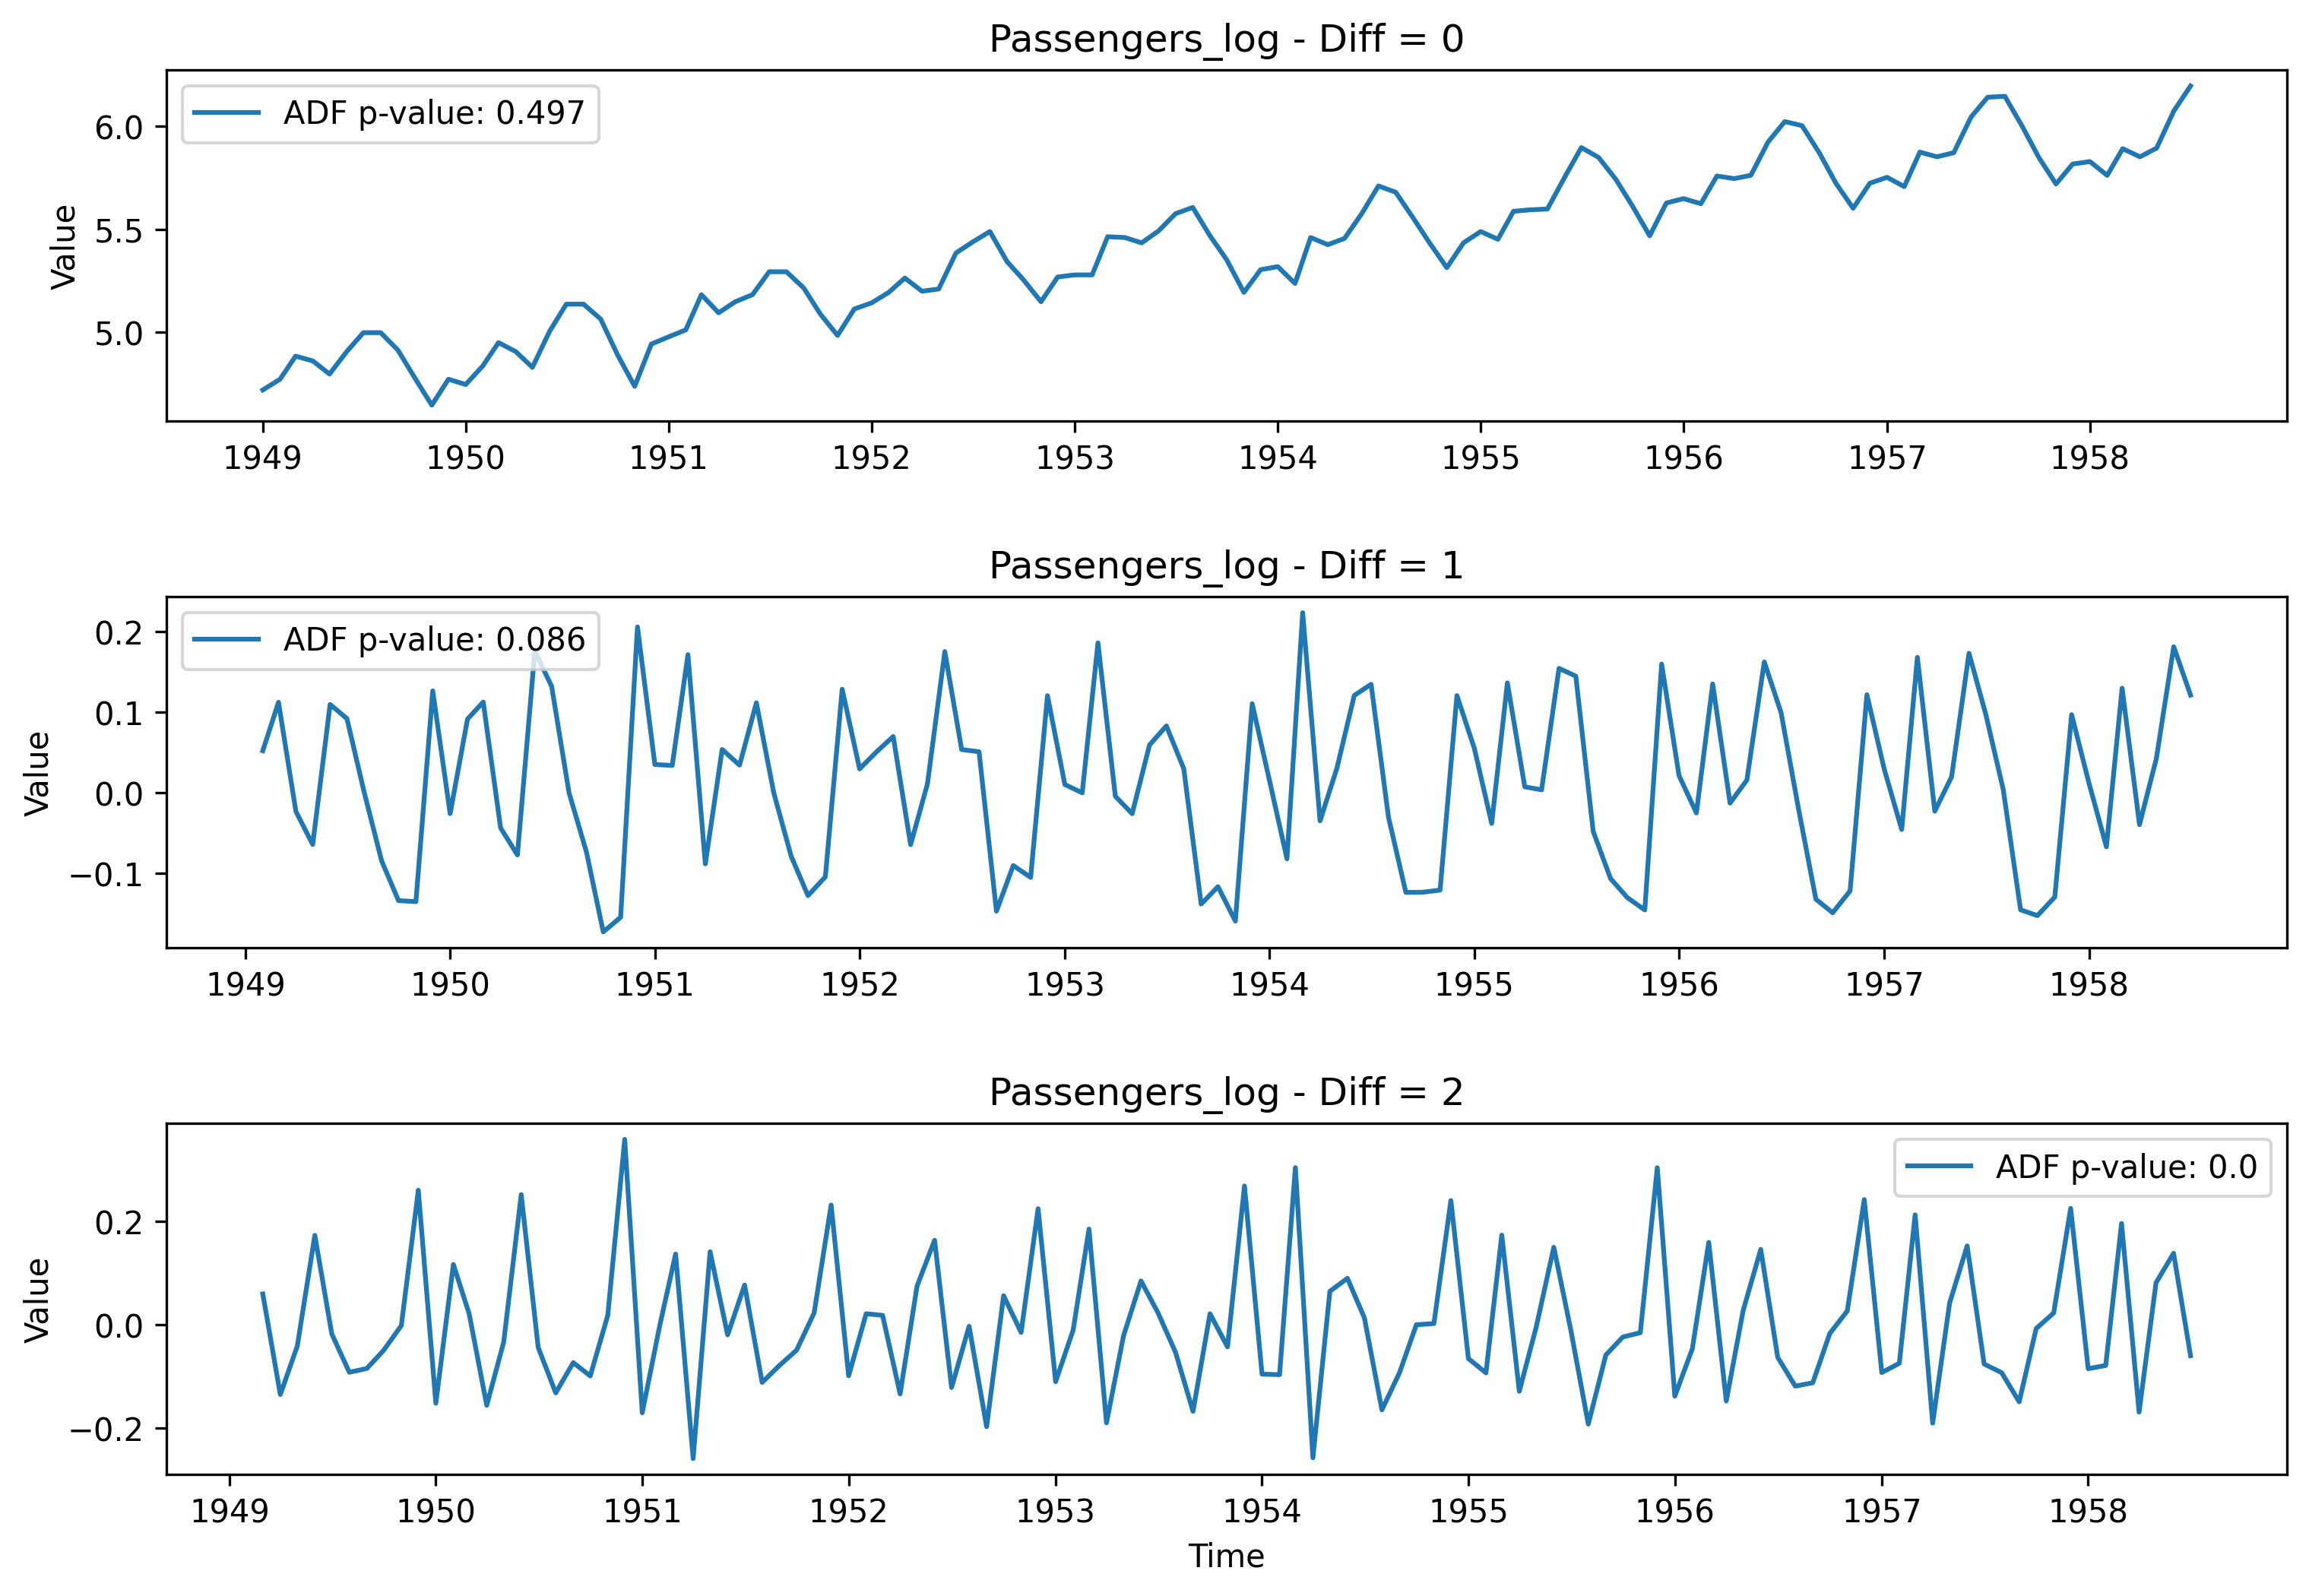
\includegraphics[scale=0.5]{notebooks/TS/img/time_series_differentiation.png}
    \caption{Time Series Differentiation Plot}
\end{figure}

Vemos que el $p$-valor en la segunda diferenciación ya es lo suficientemente pequeño para asumir estacionalidad en la serie de tiempo, así $d=2$. 

\subsection{Q Value}
Finalmente, para determinar el valor $q$ es posible ver el \textit{Autocorrelation Plot} que muestra la relación de un valor en la serie de tiempo con \textbf{todos los $p$ lags} anteriores. 
\begin{figure}[H]
    \center
    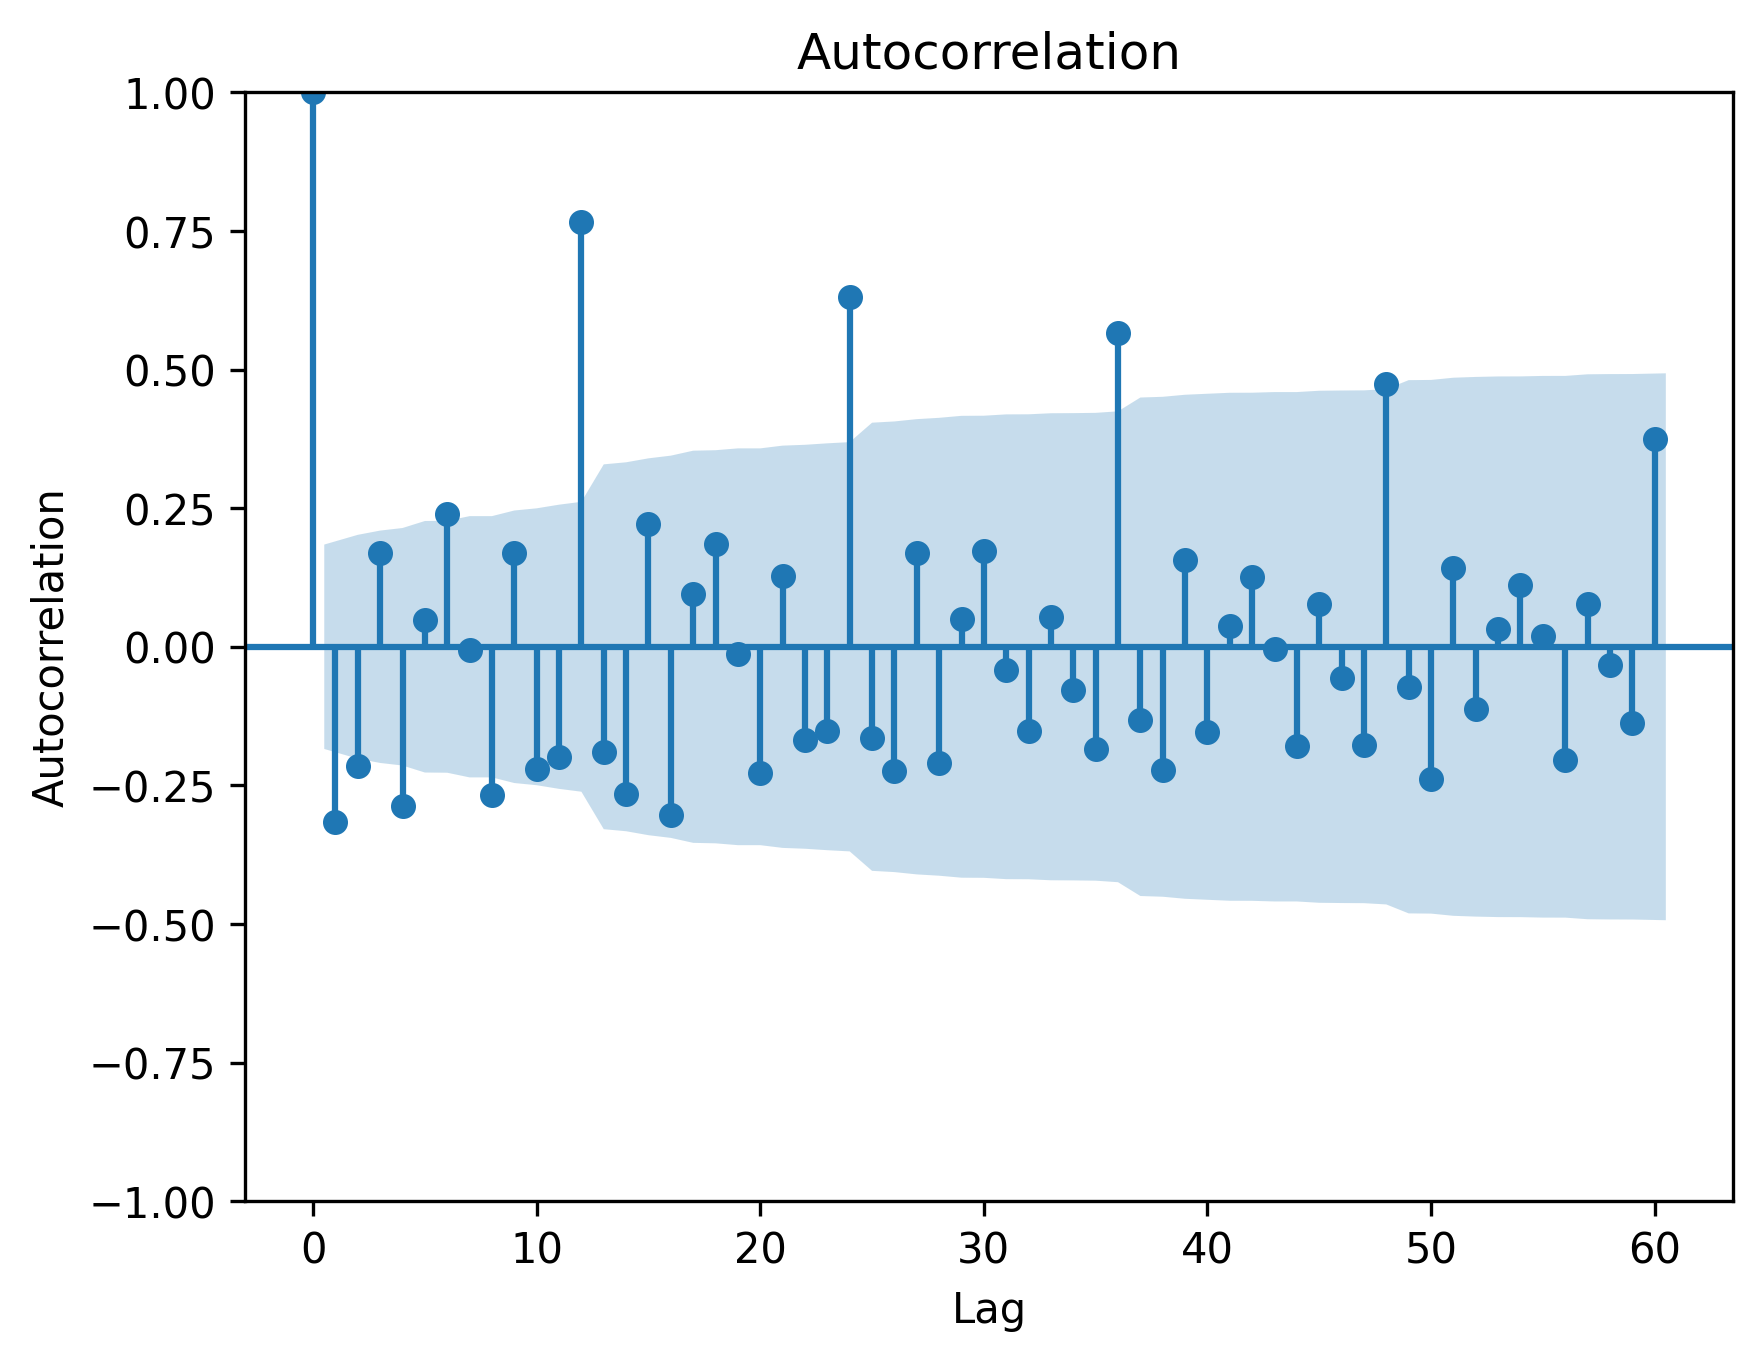
\includegraphics[scale=0.5]{notebooks/TS/img/autocorrelation.png}
    \caption{Autocorrelation Plot}
\end{figure}
En este caso, el último valor anterior a que todos los lag caigan en la zona azul, es $q=12$.
\begin{figure}[H]
    \center
    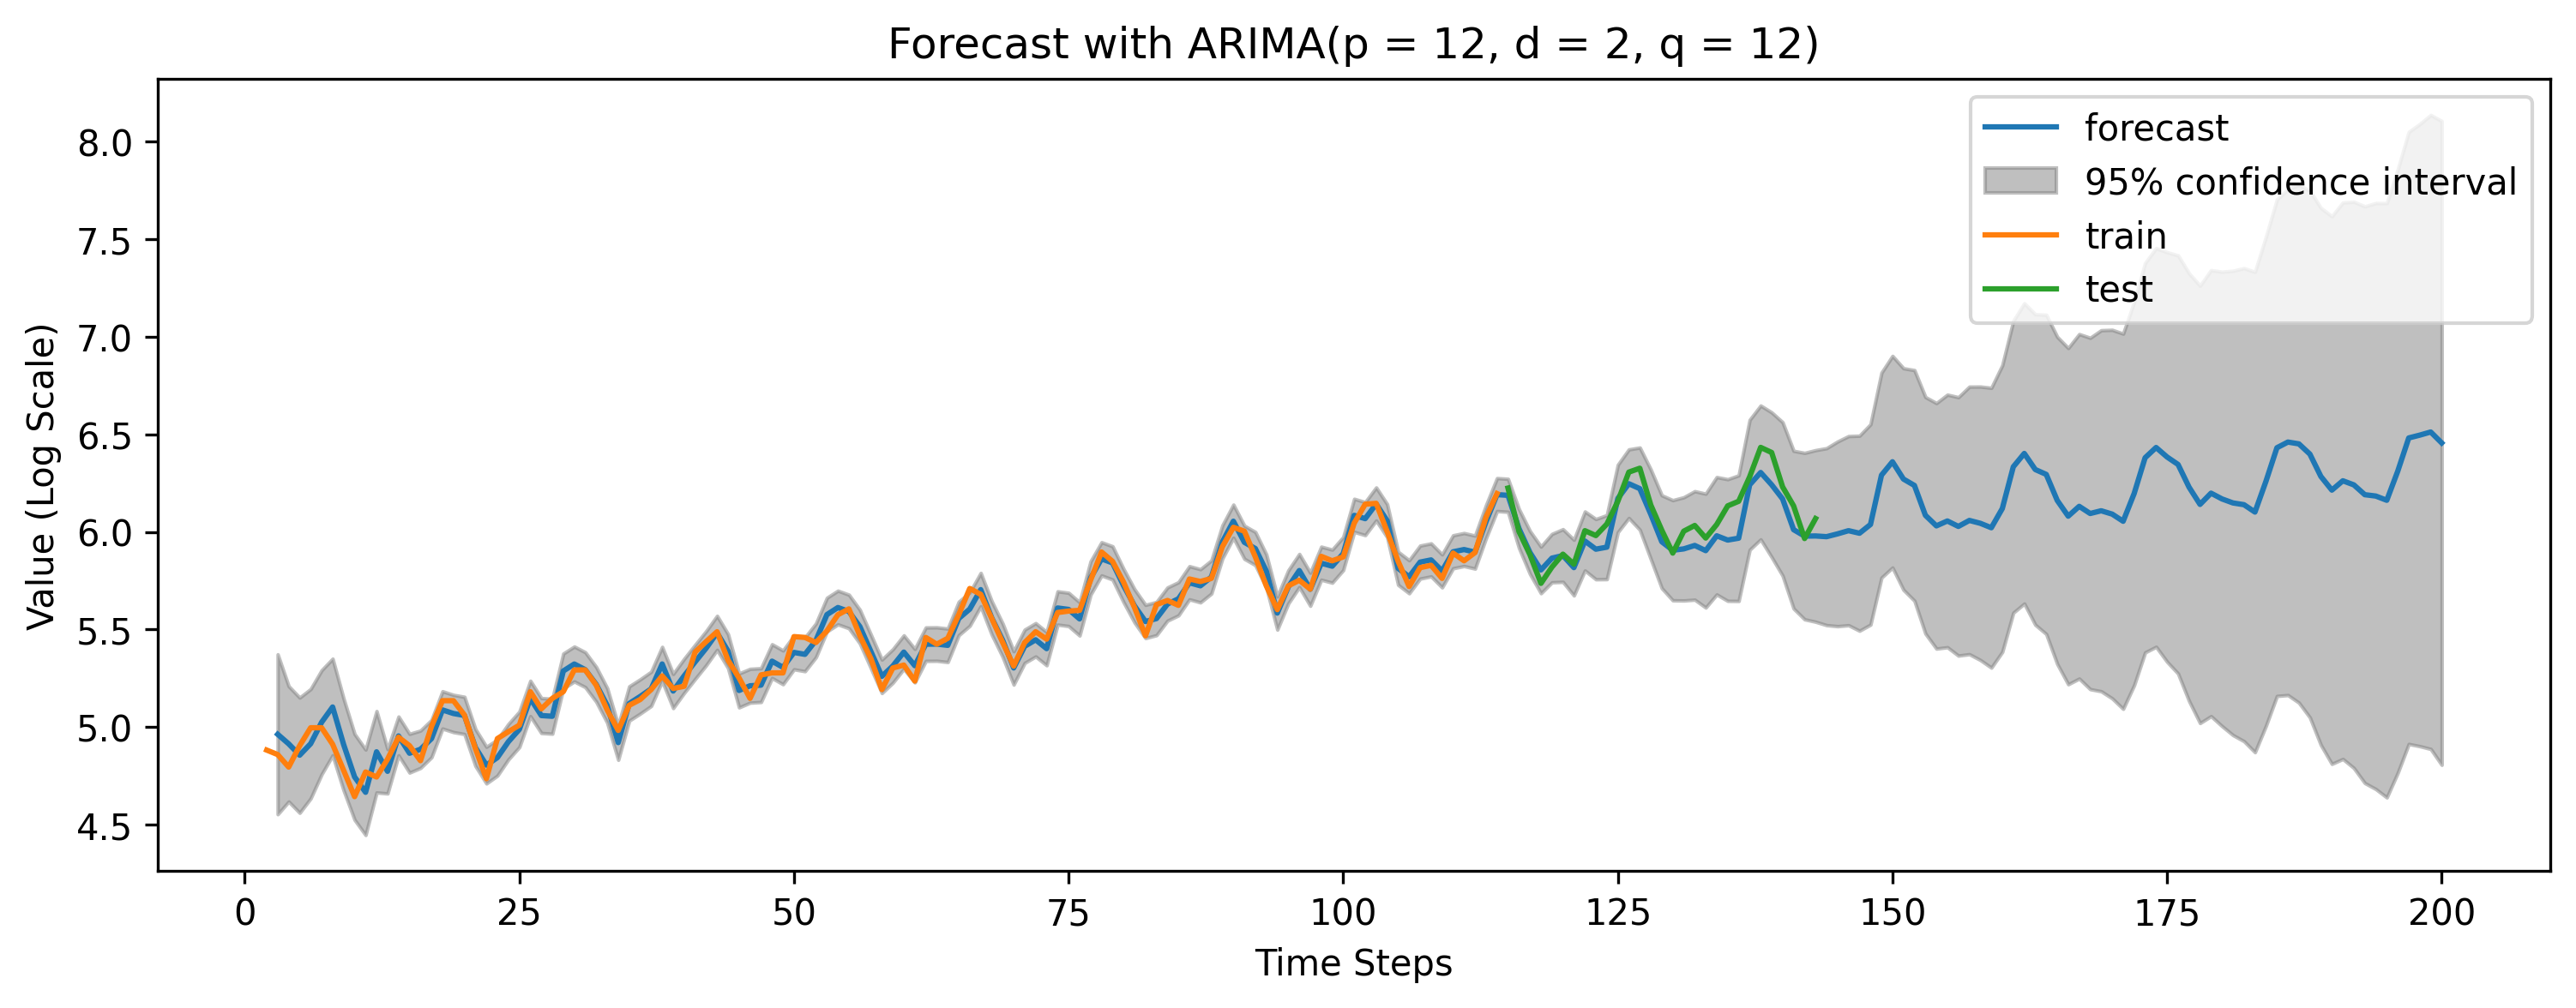
\includegraphics[scale=0.5]{notebooks/TS/img/arima_results.png}
    \caption{ARIMA over Flight Passengers Forecasting}
\end{figure}